\documentclass[french]{beamer}
\usepackage[utf8]{inputenc}
\usepackage[T1]{fontenc}
\usepackage{babel}
\usepackage{graphicx}
\usepackage{default}
\usepackage{amsfonts,amssymb}

\usetheme{metropolis}

\setbeamercolor{framesubtitle}{fg=mDarkTeal}
\addtobeamertemplate{frametitle}{}{%
  \ifx\insertframesubtitle\@empty\else%
  \usebeamerfont{framesubtitle}%
  \usebeamercolor[fg]{framesubtitle}%
  \insertframesubtitle%
  \fi%
}

\DeclareMathOperator{\If}{if}
\DeclareMathOperator{\Else}{else}


\title{Structuring the Synthesis of Heap-Manipulating Programs}

\author{NADIA POLIKARPOVA, UCSD, USA \\ILYA SERGEY, University College London, UK}

\date{}
\begin{document}
	\maketitle
\begin{frame}[fragile]
	\frametitle{Introduction}
	
	\begin{center}
		
\includegraphics[height=\baselineskip]{figures/swap.png}
	\end{center}
	\textbf{Intérêt} : Faire avancer l'état de l'art en matière de synthèse de programmes qui manipulent des pointeurs à partir de spécifications fonctionelles formelles.\\
	\textbf{Idée Clé} : Utiliser la logique de séparation.\\
	\textbf{Contributions} : Synthetic Separation Logic un systeme de preuve. Et SuSLik leur synthétiseur
\end{frame}
\begin{frame}[fragile]
	\frametitle{Spécifications pour la Synthèse}
	On utilise ici des tas symboliques.\\
	\begin{center}
	$\mathnormal{\Sigma};\mathnormal{\Gamma};\{\mathcal{P}\}\leadsto\{\mathcal{Q}\} | c$
	\end{center}
	\begin{itemize}
		\item $\mathnormal{\Gamma}$ : environnement
		\item $\mathnormal{\Sigma}$ : contexte
		\item $\mathcal{P}$,$\phi$,P : précondition, ses parties pure et spatiale
		\item $\mathcal{Q}$,$\psi$,Q : postcondition, ses parties pure et spatiale
		\item $GV(\mathrm{\Gamma},\mathcal{P},\mathcal{Q}) = Vars(\mathcal{P}) \backslash \mathnormal{\Gamma}$ 
		\item $EV(\mathnormal{\Gamma},\mathcal{P},\mathcal{Q}) = Vars(\mathcal{Q}) \backslash (\mathnormal{\Gamma} \cup Vars(\mathcal{P})$ 
	\end{itemize}
\end{frame}
\begin{frame}[fragile]
	\frametitle{Règles d'Inférence Basiques}
	\framesubtitle{Un exemple}
	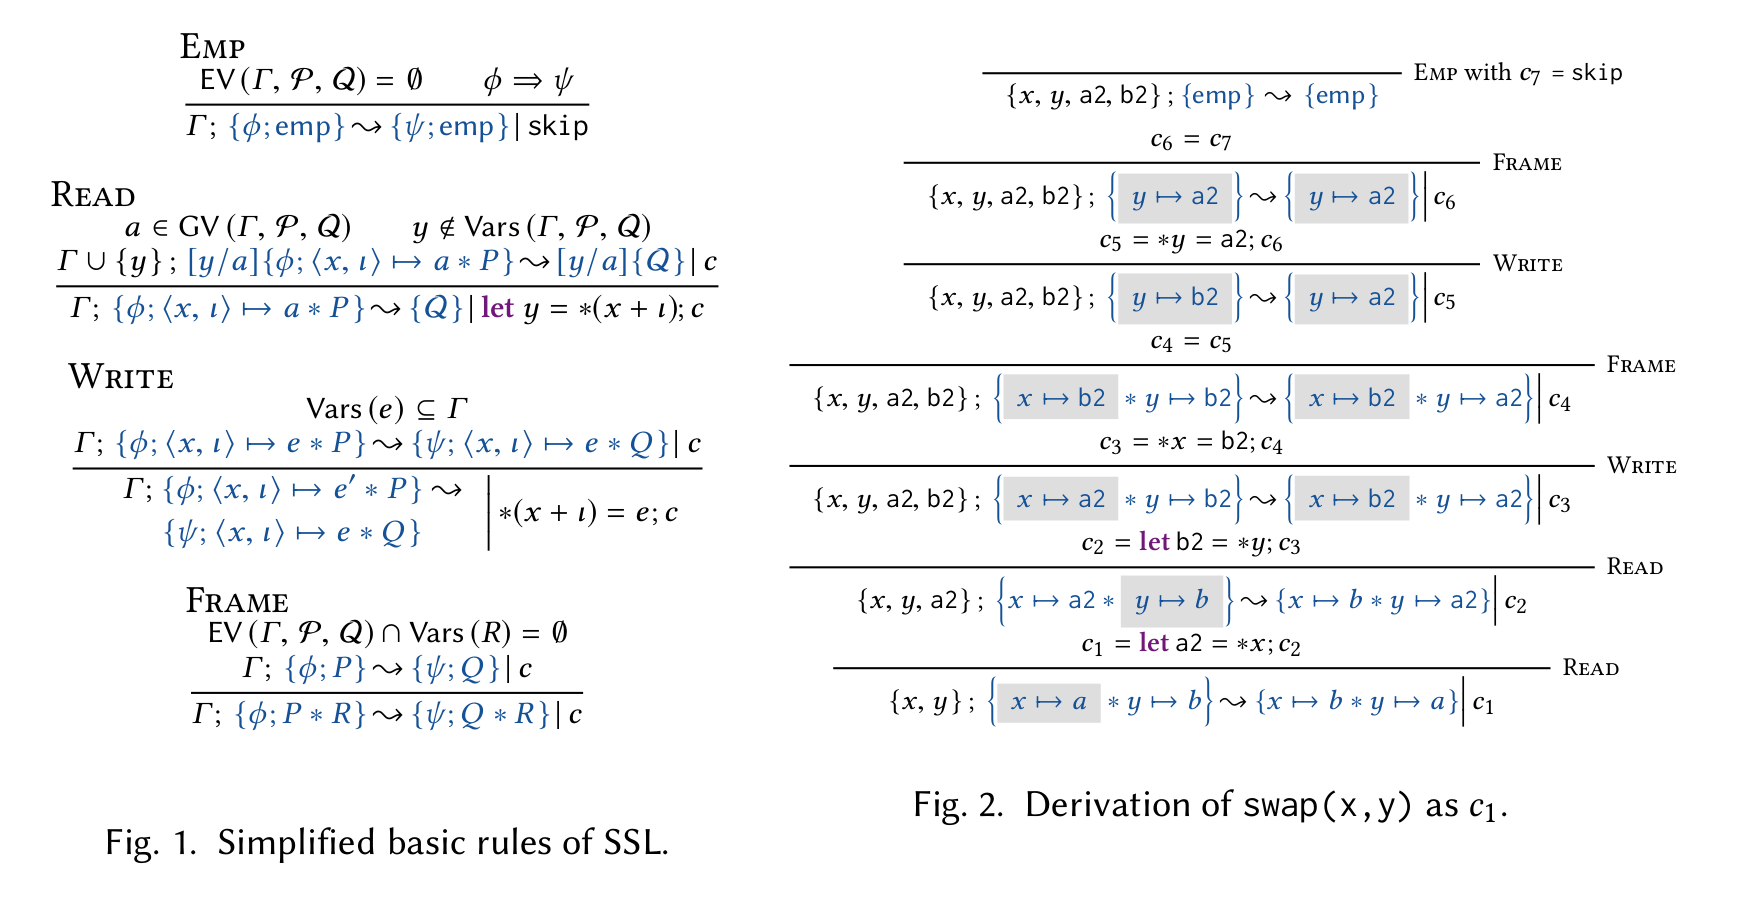
\includegraphics[width=11cm]{figures/basic.png}
\end{frame}
\begin{frame}
	\frametitle{Règles d'Inférence Basiques}
	\begin{itemize}
		\item[EMP] terminale, parties spatiales vide, $EV = \emptyset$, $\phi \implies \psi$ \\ skip
		\item[READ] assigne la valeur d'une GV a une nouvelle variable de programme et substitue toutes les occurences.\\
		let b = *x
		\item[WRITE] assigne l'évaluation d'une expression e à une case mémoire.\\
		*x = b 
		\item[FRAME] Enlève une partie spatiale commune à $\phi$ et $\psi$, si cela ne crée pas de variable existentielle.\\
		skip
	\end{itemize}
\end{frame}
\begin{frame}[fragile]
	\frametitle{Unification Spatiale et Backtrack}
   
\includegraphics[height=\baselineskip]{figures/spatial_unification.png}
   
   Avec la substitution $z \mapsto 239$, on unfie $z$ et $239$. 
   \[ 
      \{x \mapsto 239 * y \mapsto 30\} \leadsto \{x \mapsto 239 * y \mapsto 239\}.
   \]
   Introduit du déterminisme et peut alors nécessiter du backtracking !
   
   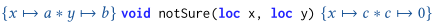
\includegraphics[height=\baselineskip]{figures/backtrack.png}
   
   Si on lit $x$ dans une variable $a_2$, on a le but (impossible)
   \[
      \{x, y, a_2\}\{y \mapsto b\} \leadsto \{a_2 \mapsto 0\}.
   \]
\end{frame}
\begin{frame}[fragile]
	\frametitle{Raisonner sur les contraintes pures}
   \framesubtitle{Précondition}
   
\includegraphics[width=\linewidth]{figures/precondition.png}
   
   Deux variables universelles égales, $x$ et $y$, on substitue.
   \[
      \{x, y\}\{y \mapsto x * x\mapsto z\} \leadsto \{x \mapsto x * x \mapsto x\}.
   \]
   Ici, mène à quelque chose d'impossible $\implies$ règle d'inconsistence ! 
\end{frame}
\begin{frame}[fragile]
	\frametitle{Raisonner sur les contraintes pures}
	\framesubtitle{Les règles}
   \centering
   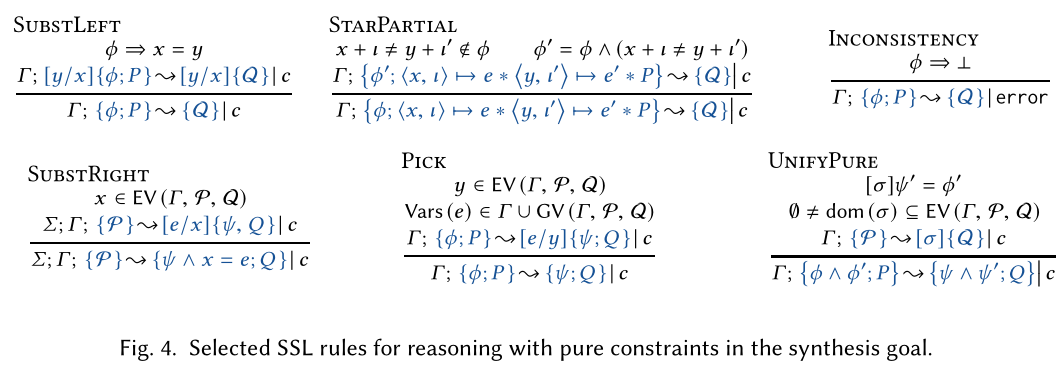
\includegraphics[width=\linewidth]{figures/pure_constraints.png}
\end{frame}


\begin{frame}[fragile]
	\frametitle{Synthèse pour prédicats inductifs}
	\framesubtitle{Mémoire dynamique}
   \begin{center}
      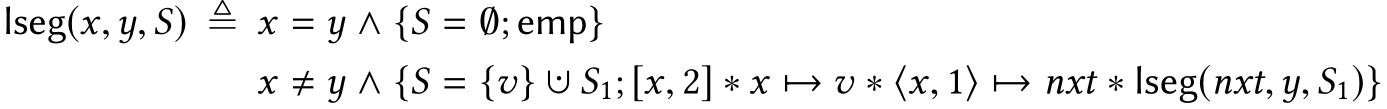
\includegraphics[width=\linewidth]{figures/lseg.png}
   Définition d'une liste chaînée dont le premier pointeur est $x$,
   le dernier $y$ et les éléments sont ceux de $S$.
   \end{center}
   On étend notre langage avec 
   \begin{itemize}   
      \item Des prédicats inductifs.
      \item Des blocs de mémoire (et ajout de règles \textsc{ALLOC} et \textsc{FREE}).
   \end{itemize}
\end{frame}

\begin{frame}[fragile]
	\frametitle{Synthèse pour prédicats inductifs}
	\framesubtitle{Induction}
   \begin{center}
      
\includegraphics[height=\baselineskip]{figures/induction1.png}
   \end{center}
   On veut synthétiser la fonction pour libérer une liste chaînée.
   
   Une règle \textsc{INDUCTION} qui 
   \begin{itemize}
      \item ajoute la fonction au contexte (permettre les appels récursifs) ;
      \item ajoute une étiquette à la fonction (utile pour la terminaison).
   \end{itemize} 
   \begin{center}
      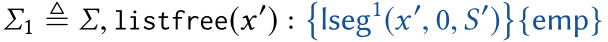
\includegraphics[height=\baselineskip]{figures/induction2.png}
   \end{center}
\end{frame}

\begin{frame}[fragile]
	\frametitle{Synthèse pour prédicats inductifs}
	\framesubtitle{Déroulement de prédicat}
   Après la règle \textsc{Induction}, une règle \textsc{Open} qui \textit{unfold}
   la définition du prédicat et génrère deux buts à résoudre.
        
   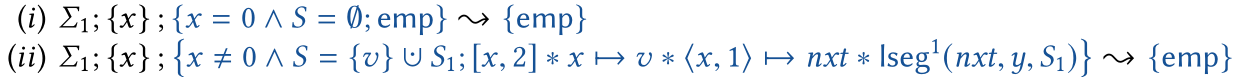
\includegraphics[width=\linewidth]{figures/unfold.png}
   
   $c_1$ et $c_2$ programmes pour (1) et (2), programme final
   \[
      \If (x = 0) \{c_1\} \Else \{ c_2 \}.
   \]
\end{frame}

\begin{frame}[fragile]
	\frametitle{Synthèse pour prédicats inductifs}
	\framesubtitle{Retour à l'étiquette de niveau}
   \begin{description}
      \item[But :] éviter les dérivations infinies (ici donne programmes qui ne terminent 
                   pas en s'appellant eux-mêmes).
      \item[Idéalement :] prédicats bien-fondés et applications récursives sur tas 
                       strictement plus petits.      
      \item[Méthode :] avec les tags, on empêche la fonction de s'appeler sur le même 
                       tas en post-condition.
   \end{description}
\end{frame}

\begin{frame}[fragile]
	\frametitle{Synthèse pour prédicats inductifs}
	\framesubtitle{Déroulement dans la postcondition}
      Si un prédicat inductif dans la postcondition.
      
      Une règle \textsc{CLOSE}.
      \begin{itemize}
         \item Choisit non déterministiquement la partie du prédicat à satisfaire.
         \item Met à jour la postconditions avec la postcondition de la partie choisie.
         \item Incrémente l'étiquette.
      \end{itemize}
\end{frame}

\begin{frame}[fragile]
	\frametitle{Permettre l'appel de procèdure}
	\framesubtitle{Enlévement de l'appel}
   
\includegraphics[width=\linewidth]{figures/abduction1.png}
   \textsc{Induction} ajoute cette fonction à l'environnement.
   
\includegraphics[width=\linewidth]{figures/abduction2.png}
   \begin{center}
      \textsc{Open} (plus d'autres règles) créent ce but.
      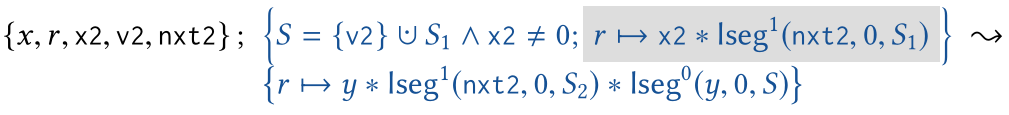
\includegraphics[width=\linewidth]{figures/abduction3.png}
      Peut pas utiliser \textsc{CALL} (il faut $r \mapsto nxt2$).
   \end{center}
   
   Solution : ajout d'une règle \textsc{AbduceCall} qui \og prépare \fg le tas.
              Essaie d'unifier les préconditions de notre but et celles de la 
              fonction qu'on veut appeler.
\end{frame}

\begin{frame}[fragile]
	\frametitle{Synthetic Separation Logic}
	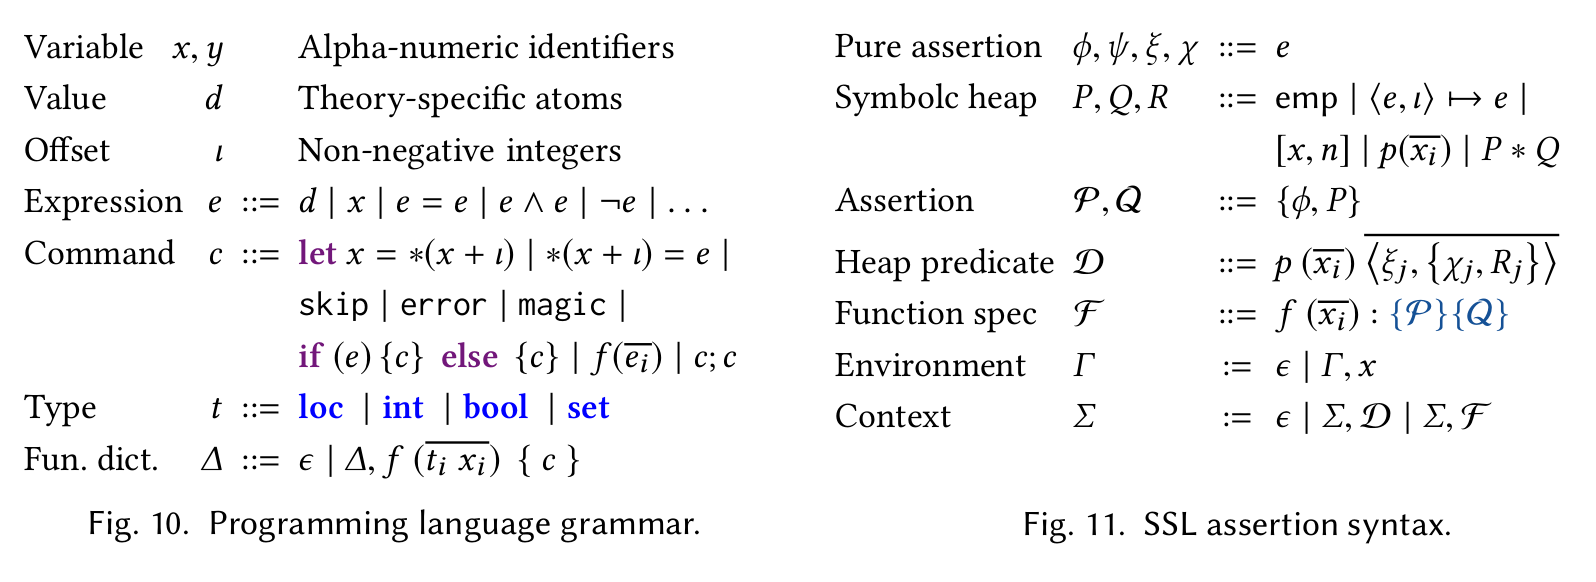
\includegraphics[width=11cm]{figures/syntax.png}
\end{frame}
\begin{frame}[fragile]
	\frametitle{Synthetic Separation Logic}
	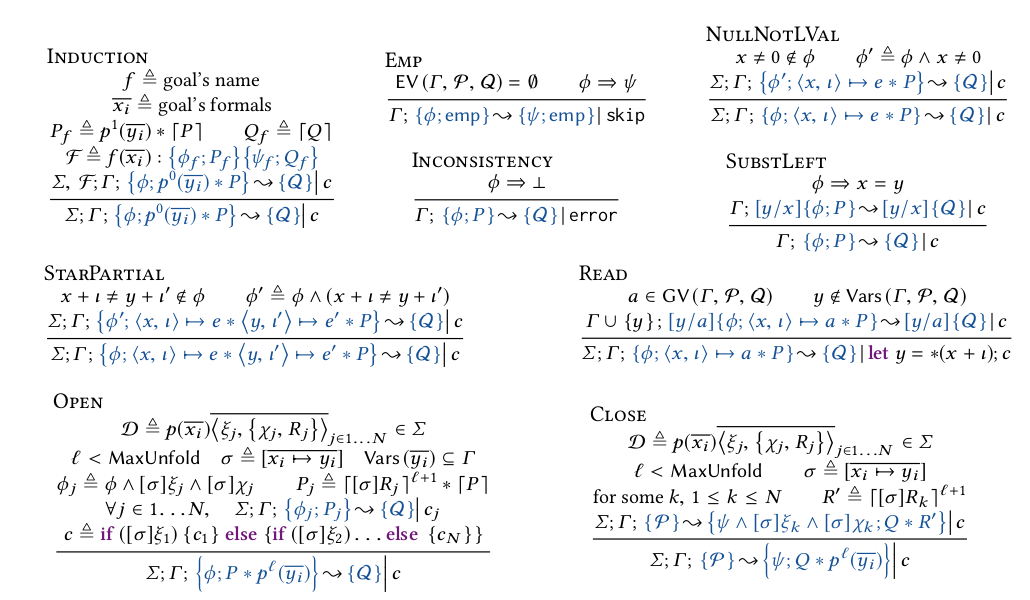
\includegraphics[width=11cm]{figures/zoo1.png}
\end{frame}
\begin{frame}[fragile]
	\frametitle{Synthetic Separation Logic}
	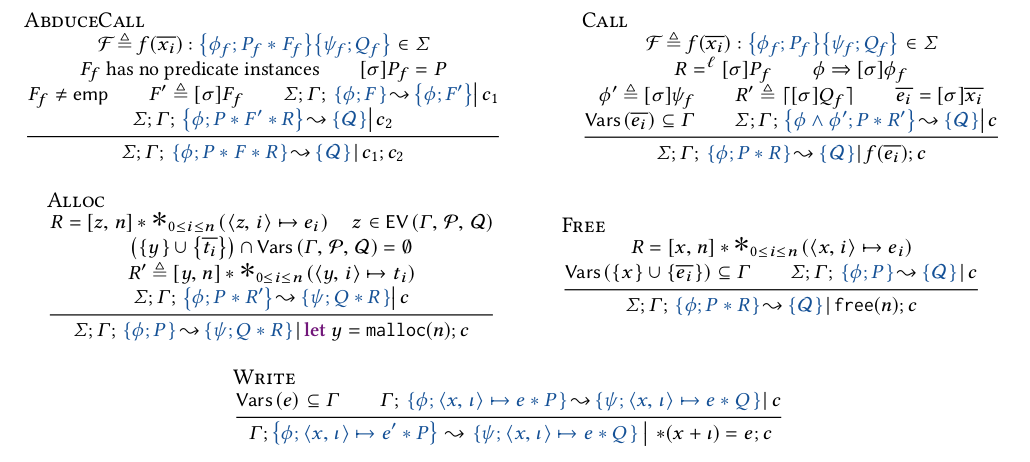
\includegraphics[width=11cm]{figures/zoo2.png}
\end{frame}
\begin{frame}[fragile]
	\frametitle{Synthetic Separation Logic}
	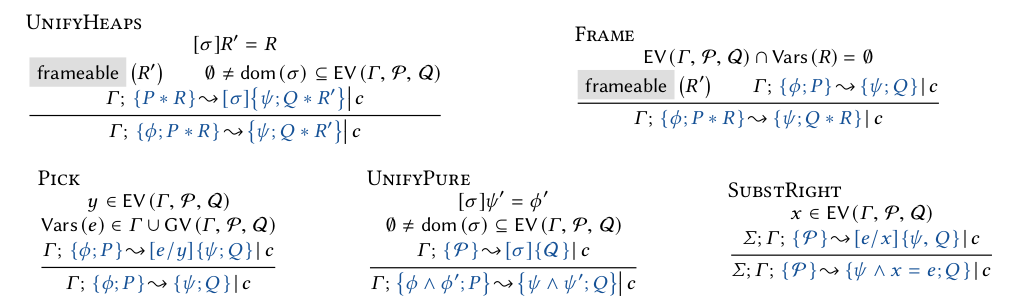
\includegraphics[width=11cm]{figures/zoo3.png}
\end{frame}
\begin{frame}[fragile]
	\frametitle{Garanties Formelles}
	La validité pour la partie SL est assez similaire au cas plus classique.\\
	\vspace{0.5cm}
	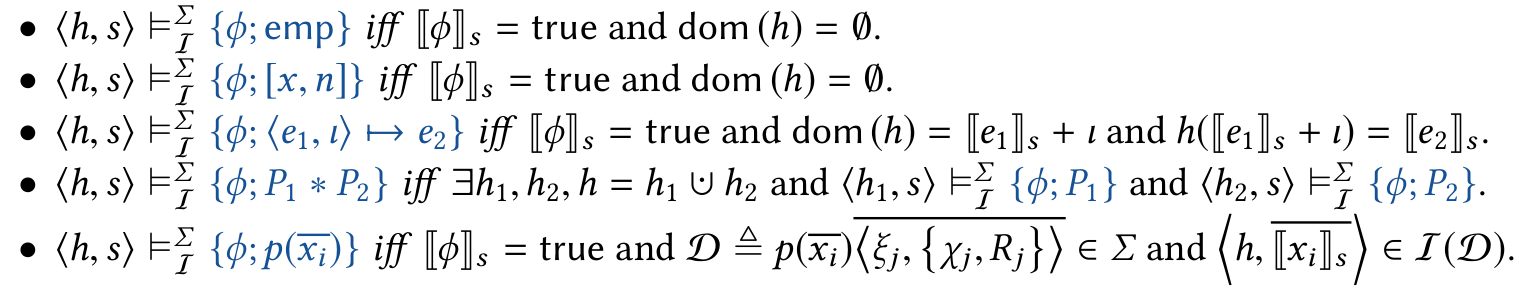
\includegraphics[width=11cm]{figures/satisfaction.png}
\end{frame}
\begin{frame}[fragile]
	\frametitle{Garanties Formelles}
	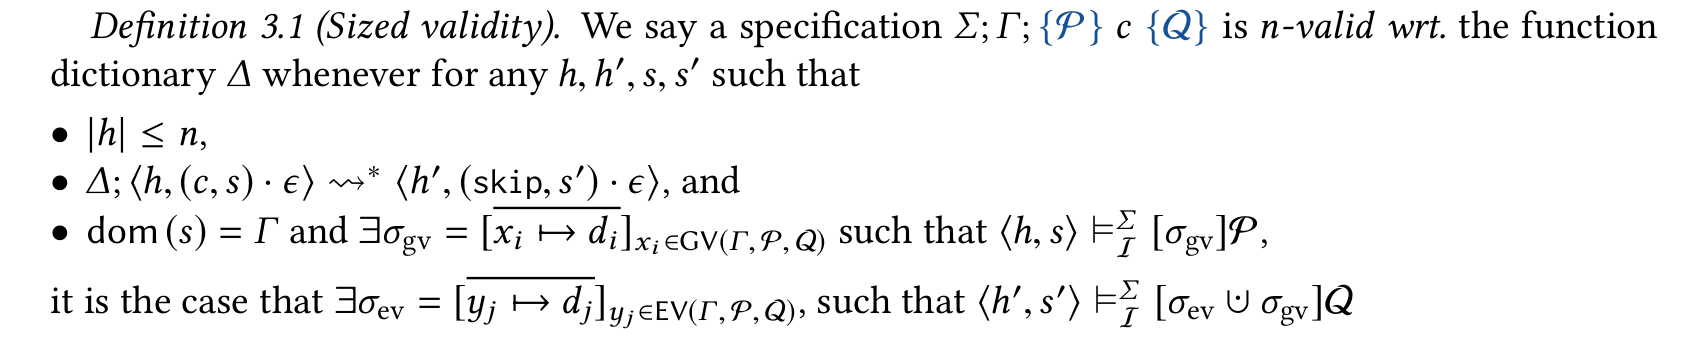
\includegraphics[width=11cm]{figures/nvalid.png}\\
	
	On définit une validité vis à vis de la pré et post condition mais seulement pour des tas de taille n.
\end{frame}
\begin{frame}[fragile]
	\frametitle{Garanties Formelles}
	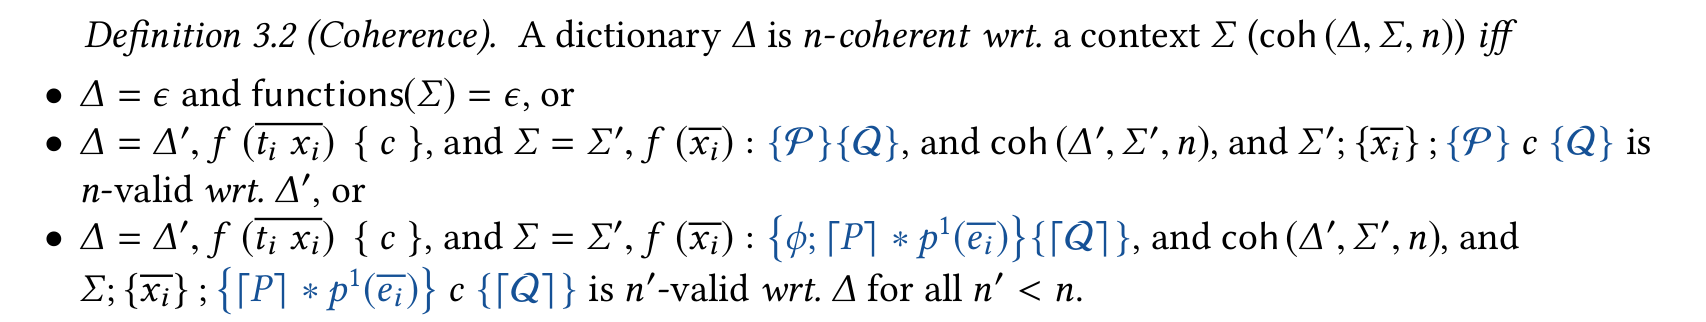
\includegraphics[width=11cm]{figures/coherence.png}
\end{frame}
\begin{frame}[fragile]
	\frametitle{Garanties Formelles}
	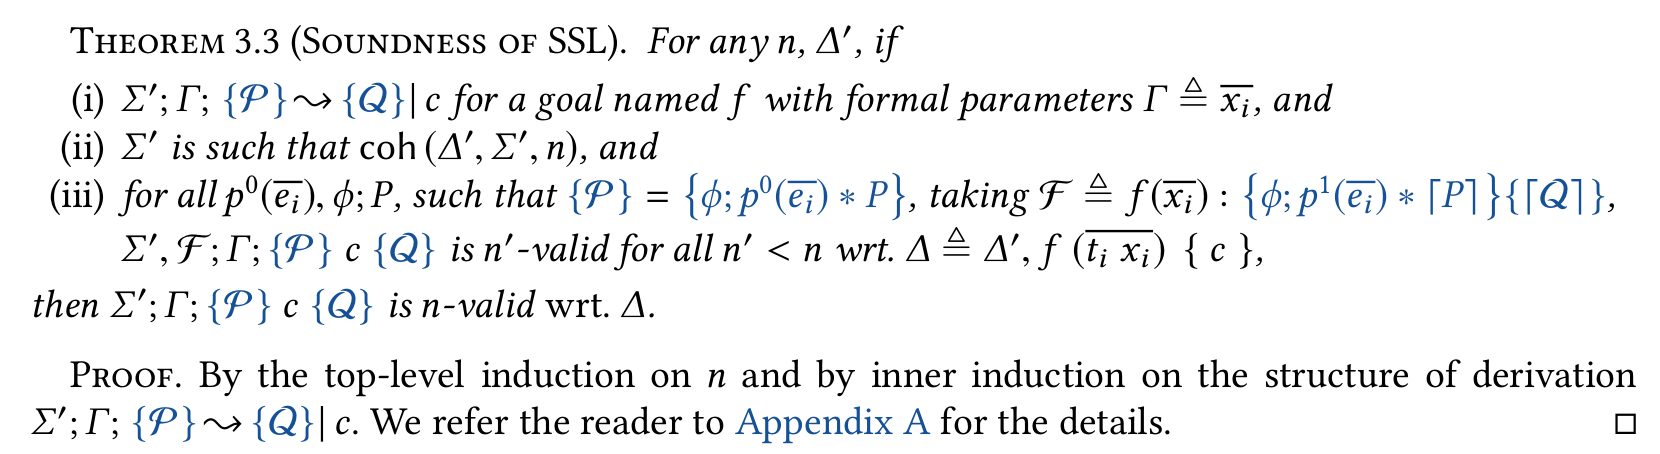
\includegraphics[width=11cm]{figures/thm.png}
\end{frame}
\begin{frame}[fragile]
	\frametitle{Algorithme de synthèse basé sur SSL}
\end{frame}
\begin{frame}[fragile]
	\frametitle{Optimisations et extensions}
	Optimisations :
	\begin{itemize}
		\item Règles inversibles
		\pause
		\item Recherche multi-phase
		\pause
		\item Rèduction des symétries
		\pause
		\item Règles d'échec 
	\end{itemize}
	\pause
	Extensions :
	\begin{itemize}
	\item Fonctions auxilliaire
	\pause
	\item Enlèvement de branches	
	\end{itemize}
\end{frame}
\begin{frame}
	\frametitle{Benchmark}
	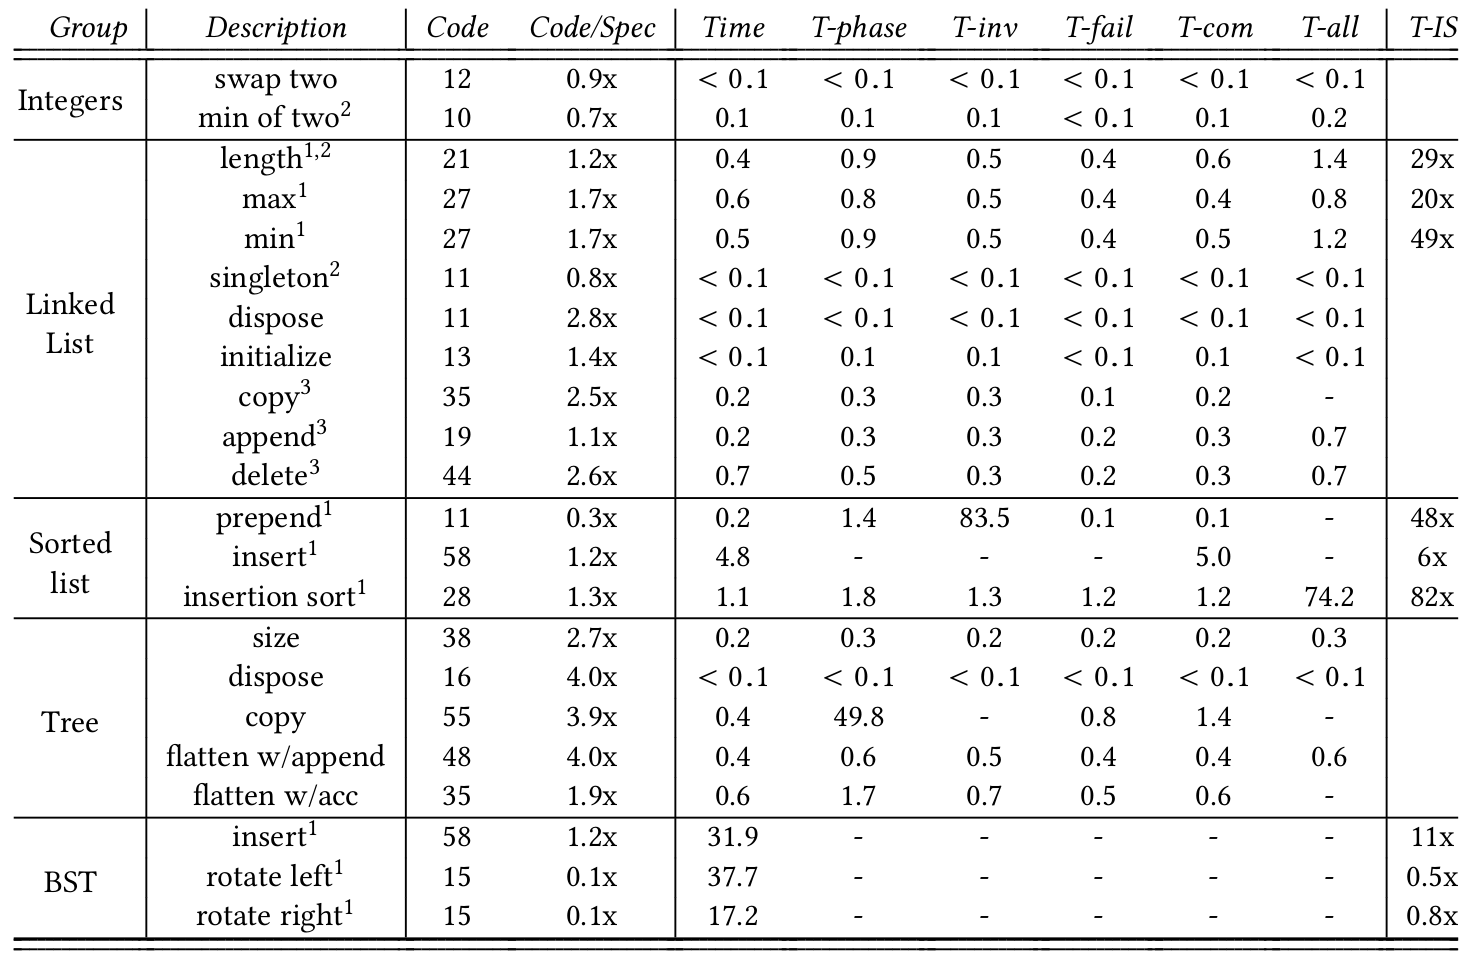
\includegraphics[width=11cm]{figures/benchmark.png}
\end{frame}


\end{document}
